\section{Results: What History Reads}
\label{sec:results-mechanism}

% src: diagnostics_2026_10/{baseline_uniform_nlos,mixed_propagation}/history_mechanism_diagnostic_summary.json (5 seeds 42/1/7/13/99; models xgboost, random_forest, knn; conditions pure_snap, snap, rss_hist, angle_hist, ray_hist, full; gains seed-paired against snap)
In the macro-cell study, the gain from history is carried almost entirely by the angle channels, and what it mainly reduces is range error. The test fed $k$-NN, Random Forest and XGBoost history for one group of channels at a time while keeping every other channel at its current value: the RSS group~(RSS, SINR and the RSS difference), the angle group~(the sines and cosines of both angles and the azimuth difference), or the ray group~(the two ray-projection coordinates and their differences). All conditions use the same samples and the same five user splits as the full $h=5$ input, so every comparison is paired, and none of these models selects anything on the test users. The test ran on both the uniform-NLOS and the mixed-propagation realizations.

\begin{figure}[h]
  \centering
  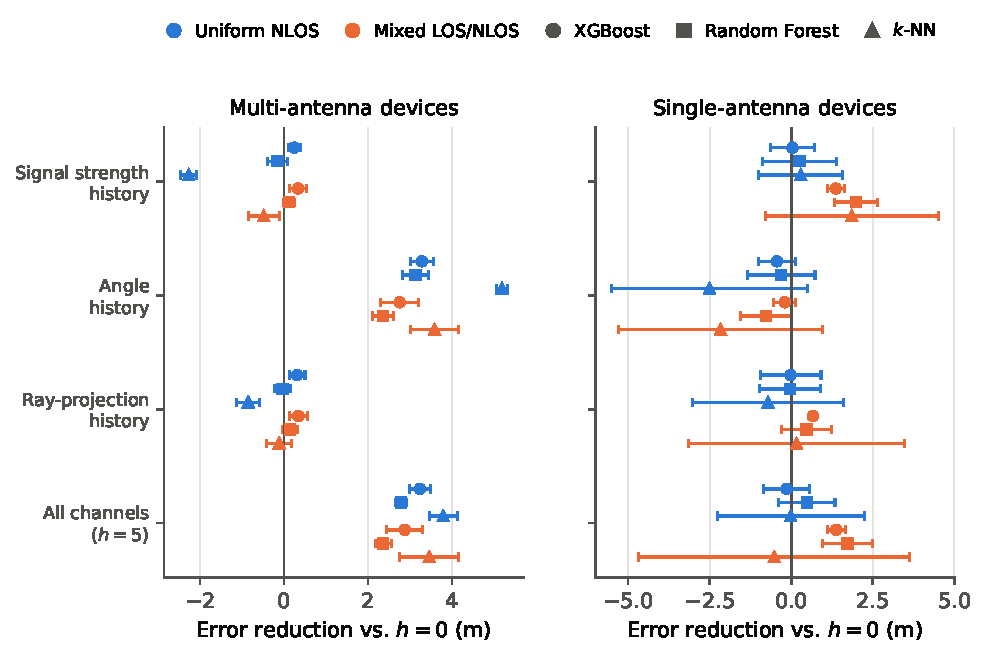
\includegraphics[width=0.95\textwidth]{fig_mechanism_conditions}
  \caption{Reduction in mean error against the $h=0$ input when history is given to one channel group at a time, or to all channels, per device group, model and dataset. Seed-paired means over five user splits with $95\%$ confidence intervals.}
  \label{fig:mechanism-conditions}
\end{figure}
% src: figure_scripts/make_figures_diagnostic.py mechanism_conditions()

% src: summary.<model>.angle_hist / rss_hist / ray_hist / full .multi.gain_vs_snap (uniform: XGB 3.28+-0.27 / 0.25+-0.14 / 0.31+-0.19 / 3.24+-0.26; RF 3.14+-0.30 / -0.15+-0.23 / -0.04+-0.18 / 2.79+-0.13; kNN 5.19+-0.12 / -2.27+-0.19 / -0.85+-0.27 / 3.79+-0.33; mixed angle: XGB 2.76+-0.45, RF 2.36+-0.25, kNN 3.59+-0.57)
The first prediction holds without exception~(Figure~\ref{fig:mechanism-conditions}). For multi-antenna devices on the uniform-NLOS data, angle history alone lowered error by $3.28 \pm 0.27\,\text{m}$ for XGBoost and $3.14 \pm 0.30\,\text{m}$ for Random Forest, as much as history on every channel~($3.24$ and $2.79\,\text{m}$). RSS history alone gave $0.25 \pm 0.14\,\text{m}$ for XGBoost and nothing detectable for Random Forest, and ray history behaved the same way. For $k$-NN, angle history alone outperformed the full window~($5.19$ against $3.79\,\text{m}$), and RSS history made it worse by $2.27\,\text{m}$, consistent with uninformative lags adding noise to its distance metric. The mixed-propagation data repeat the pattern, with angle-only gains of $2.4$ to $3.6\,\text{m}$ across the three models.

% src: per_seed.xgboost.{snap,full}.groups.multi radial_mean / tangential_mean (5-seed means 17.31 -> 14.12, 5.02 -> 4.60); single 20.23 -> 20.13, 25.22 -> 25.29
What the angle history improves is mainly the estimate of distance~(Figure~\ref{fig:radial-tangential}). For multi-antenna devices, five steps of history lowered XGBoost's mean radial error from $17.3$ to $14.1\,\text{m}$ and its tangential error only from $5.0$ to $4.6\,\text{m}$. Bearing was already well determined by the current angle measurement; the sequence of angles adds information about range. This is what Equation~(\ref{eq:dtheta-dt}) allows: for a given sideways movement, the rate at which the bearing turns falls as $1/r$, so a window of bearings carries information about distance that a single bearing does not. Single-antenna devices show no change in either component.

\begin{figure}[h]
  \centering
  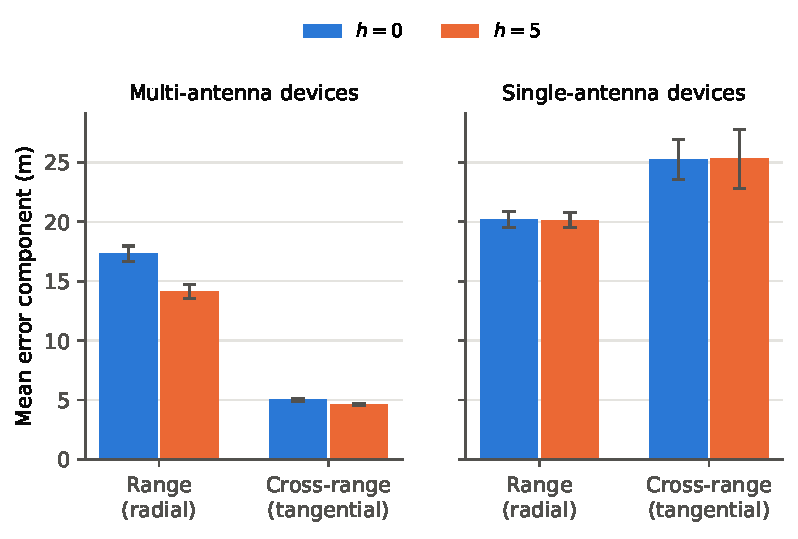
\includegraphics[width=0.75\textwidth]{fig_radial_tangential}
  \caption{Mean radial~(range) and tangential~(cross-range) components of the position error without history~($h=0$) and with five steps~($h=5$), per device group, XGBoost, macro-cell study. Means over five seeds; bars are $95\%$ confidence intervals.}
  \label{fig:radial-tangential}
\end{figure}
% src: figure_scripts/make_figures_diagnostic.py radial_tangential()

% src: summary.<model>.pure_snap.multi.gain_vs_snap (uniform: XGB -0.49+-0.14, RF -0.40+-0.21, kNN -0.33+-0.54)
The test also measures how much history the $h=0$ input already contains. Removing the first differences from the $h=0$ input raised multi-antenna error by $0.49 \pm 0.14\,\text{m}$ for XGBoost and $0.40 \pm 0.21\,\text{m}$ for Random Forest. The history gains reported in Section~\ref{sec:results-multi} are therefore measured against a baseline that already holds one step of change, and they understate the full effect of history by roughly $15\%$.

% src: summary.<model>.<cond>.single.gain_vs_snap (uniform: all CIs include zero, e.g. XGB full -0.14+-0.70; mixed: XGB rss_hist 1.36+-0.26, full 1.38+-0.27; RF rss_hist 1.99+-0.66, full 1.73+-0.77; per-seed XGB rss_hist 1.27/1.29/1.10/1.28/1.87); mixed_propagation_2026_09/seed_repeats_all_models_summary.json (single h0->h5 paired: XGB 1.66+-0.50, RF 1.55+-0.73, 1D-CNN -1.00+-0.71)
The second prediction holds on the uniform-NLOS data and fails on the mixed-propagation data. Under uniform NLOS, no channel group lowered single-antenna error for any model; every confidence interval includes zero. With mixed propagation, RSS history lowered single-antenna error for both tree ensembles, by $1.36 \pm 0.26\,\text{m}$ for XGBoost and $1.99 \pm 0.66\,\text{m}$ for Random Forest, and the gain was positive in every one of the five splits. The separate five-seed comparison of all seven models on the mixed data confirms this for the two tree ensembles, but the neural models do not share it, and the 1D-CNN's single-antenna error rises slightly with history. Section~\ref{sec:results-propagation} examines where this gain arises.

\begin{figure}[h]
  \centering
  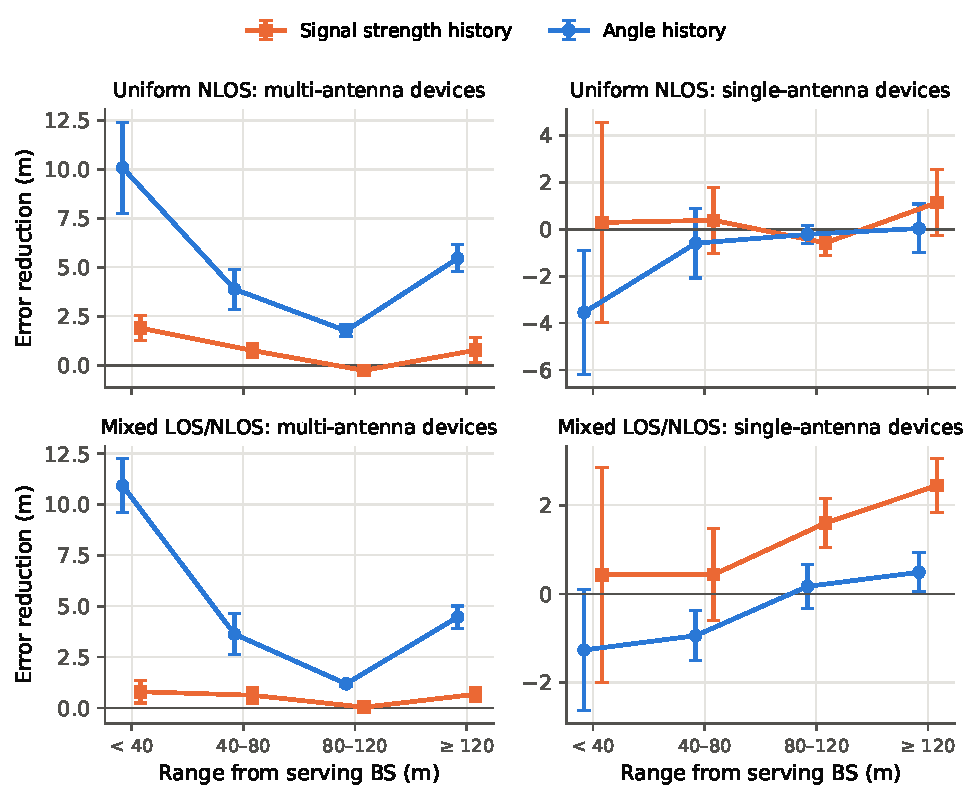
\includegraphics[width=0.85\textwidth]{fig_mechanism_by_range}
  \caption{Reduction in mean error against the $h=0$ input by range from the serving BS, for RSS-only and angle-only history, per device group and dataset, XGBoost. Seed-paired means over five user splits with $95\%$ confidence intervals. The nearest band holds about $160$ single-antenna test samples per split.}
  \label{fig:mechanism-by-range}
\end{figure}
% src: figure_scripts/make_figures_diagnostic.py mechanism_by_range(); summary.xgboost.{rss_hist,angle_hist}.*.gain_vs_snap_by_range

% src: summary.xgboost.rss_hist.multi.gain_vs_snap_by_range (uniform: <40 1.90, 40-80 0.75, 80-120 -0.26, >=120 0.77); summary.random_forest.rss_hist.multi (uniform: -0.87, 0.53, -0.39, -0.26); summary.xgboost.rss_hist.single (mixed: 0.43, 0.44, 1.60, 2.44); summary.xgboost.angle_hist.multi (uniform: 10.09, 3.89, 1.76, 5.46)
The third prediction is not supported~(Figure~\ref{fig:mechanism-by-range}). If RSS history were limited by the shrinking gradient of Equation~(\ref{eq:rss-gradient}), its gain should be largest near the BS and fall with range. For multi-antenna devices on the uniform-NLOS data, XGBoost's RSS-only gain does fall from $1.9\,\text{m}$ within $40\,\text{m}$ to slightly below zero at $80$ to $120\,\text{m}$, but it rises again beyond $120\,\text{m}$, and Random Forest shows no trend at all. For single-antenna devices on the uniform-NLOS data, too few samples lie near the BS to decide. On the mixed-propagation data, the single-antenna RSS-only gain runs the opposite way, rising from $0.4\,\text{m}$ near the BS to $2.4\,\text{m}$ beyond $120\,\text{m}$. The range-dependent account of Section~\ref{subsec:hypothesis} therefore does not explain when RSS history helps. Its other half, that the macro-cell gain depends on the angle channels, is the part the test confirms.

The angle-only gain is itself strongly range-dependent. For multi-antenna devices it falls from about $10\,\text{m}$ within $40\,\text{m}$ of the BS to under $2\,\text{m}$ at $80$ to $120\,\text{m}$, as expected if the bearing turns more slowly with distance, and then rises again to $5.5\,\text{m}$ beyond $120\,\text{m}$, where the baseline error is also largest. The rise in the farthest band is not explained by the account above.
